\chapter{Álgebra (Matrices y vectores)}

\section{Matrices}

\paragraph{Definición de matriz}

\paragraph{Operaciones con matrices}

\subparagraph{Traspuesta}

Ejercicio: \textbf{Demuestra que cualquier matriz puede escribirse como suma de una matriz simétrica y otra antisimétrica}

\subparagraph{Producto de matrices}

\subsection{Matriz inversa}
Se puede calcular de 3 formas. Definición, Gauss-Jordan y matriz adjunta. Vamos a ver ahora los 2 primeros métodos.

\paragraph{Definición y propiedades}

\subsection{Algunas ecuaciones matriciales sencillas}

\paragraph{Gauss-Jordan}
La base del método de Gauss es que toda transformación lineal de Gauss se puede expresar como una matriz. Simplemente buscamos la matriz que transforma la matriz dada en la identidad. Para ello, ponemos la identidad a la derecha. (Espero que leyendo esta explicación te hayas enterado)


\subsection{Utilidades: Grafos}

\section{Determinantes}

\begin{defn}[Determinante]
$\appl{|\;\;|}{\mathcal{M}_n}{\real}$
\end{defn}

\subsection{Cálculo de determinantes de orden 3}

\subsection{Propiedades}

\subsection{Cálculo de determinantes de orden 4 o más}

\paragraph{Menores, Gauss}

\subsection{Matriz inversa por determinantes}

\subsection{Ecuaciones matriciales a tope}

\subsection{Rango}
\paragraph{Gauss}

\paragraph{Determinantes}

Si $|A| \neq 0$, significa que no hay 2 filas (ni 2 columnas) linealmente independientes. Si las hubiera, $|A| = 0$.

Por lo tanto, si $|A|\neq 0 \dimplies rg(A) = \text{ máx}$

¿Qué ocurre si $A\not\in\mathcal{M}_n$?

\begin{example}
\[
    A=\begin{pmatrix}2&2&3&4\\4&4&2&1\end{pmatrix}
\]

En este ejemplo, cogiendo $\left|\begin{matrix}2&2\\4&4\end{matrix}\right| = 0$, pero $\left|\begin{matrix}3&4\\2&1\end{matrix}\right| \neq 0$, por lo que estas 2 filas tienen que ser linealmente independientes, por lo que la matriz tiene rango 2.

También valdría argumentarlo desde $\left|\begin{matrix}2&3\\4&2\end{matrix}\right| \neq 0$
\end{example}

\begin{prop}[Cálculo del rango por menores]
Sea $M_p$ un menor de orden $p$ de la matriz $A\in\mathcal{M}_{n\times m}$
\[\exists M^p \tlq M_p \neq 0 \dimplies rg(A) \geq p\]
\[\forall M^p \;\; M_p = 0 \dimplies rg(A) < p\]
\end{prop}

\subsubsection{Matriz de Vandermonde}
\[
V=\begin{bmatrix}
1 & \alpha_1 & \alpha_1^2 & \dots & \alpha_1^{n-1}\\
1 & \alpha_2 & \alpha_2^2 & \dots & \alpha_2^{n-1}\\
1 & \alpha_3 & \alpha_3^2 & \dots & \alpha_3^{n-1}\\
\vdots & \vdots & \vdots & \ddots &\vdots \\
1 & \alpha_n & \alpha_n^2 & \dots & \alpha_n^{n-1}\\
\end{bmatrix}\]

\paragraph{Determinante: } El determinante se calcula con la siguiente fórmula:

\[\begin{vmatrix} V \end{vmatrix}=\prod_{1 \le i<j\le n}(\alpha_j-\alpha_i)\]

\begin{example}
\[
\begin{vmatrix}
1&2&4&8\\
1&3&9&27\\
1&4&16&64\\
1&5&25&125
\end{vmatrix} = \underbrace{\overbrace{(3-2)}^{j=2}\overbrace{(4-2)}^{j=3}\overbrace{(5-2)}^{j=4}}_{i=1}\underbrace{\overbrace{(4-3)}^{j=3}\overbrace{(5-3)}^{j=4}}_{i=2}\underbrace{\overbrace{(5-4)}^{j=4}}_{i=3} = 1·2·3·1·2·1 = 6
\]
\end{example}

\begin{proof}[por Inducción]

\paragraph{Base: n=2} Es fácil notar que en el caso de una matriz de 2×2 el resultado es correcto.
\[\begin{vmatrix} V \end{vmatrix}=v_{1,1}v_{2,2} - v_{1,2}v_{2,1}=\alpha_2-\alpha_1=\prod_{1\le i<j\le 2} (\alpha_j-\alpha_i)\]

\paragraph{Paso}
Suponiendo cierta la fórmula para el caso $n-1$, procedemos a calcular el determinante de orden $n$. Para ello, basta con realizar la siguiente operación elemental sobre cada columna: $C_{j}\rightarrow C_{j}-(\alpha_1 \times C_{j-1})$. Esta operación no afecta al determinante, por lo que se obtiene lo siguiente:

\[
\begin{vmatrix} V \end{vmatrix}=\begin{vmatrix}
1 & \alpha_1 & \alpha_1^2 & \dots & \alpha_1^{n-1}\\
1 & \alpha_2 & \alpha_2^2 & \dots & \alpha_2^{n-1}\\
1 & \alpha_3 & \alpha_3^2 & \dots & \alpha_3^{n-1}\\
\vdots & \vdots & \vdots & \ddots &\vdots \\
1 & \alpha_n & \alpha_n^2 & \dots & \alpha_n^{n-1}\\
\end{vmatrix}=\begin{vmatrix}
1 & 0 & 0 & \dots & 0\\
1 & \alpha_2-\alpha_1 & \alpha_2(\alpha_2-\alpha_1) & \dots & \alpha_2^{n-2}(\alpha_2-\alpha_1)\\
1 & \alpha_3-\alpha_1 & \alpha_3(\alpha_3-\alpha_1) & \dots & \alpha_3^{n-2}(\alpha_3-\alpha_1)\\
\vdots & \vdots & \vdots & \ddots &\vdots \\
1 & \alpha_n-\alpha_1 & \alpha_n(\alpha_n-\alpha_1) & \dots & \alpha_n^{n-2}(\alpha_n-\alpha_1)\\
\end{vmatrix}
\]

Desarrollando por los adjuntos de la primera fila: 

\[\begin{vmatrix} V \end{vmatrix}=\begin{vmatrix}
\alpha_2-\alpha_1 & \alpha_2(\alpha_2-\alpha_1) & \dots & \alpha_2^{n-2}(\alpha_2-\alpha_1)\\
\alpha_3-\alpha_1 & \alpha_3(\alpha_3-\alpha_1) & \dots & \alpha_3^{n-2}(\alpha_3-\alpha_1)\\
\vdots & \vdots & &\vdots \\
\alpha_n-\alpha_1 & \alpha_n(\alpha_n-\alpha_1) & \dots & \alpha_n^{n-2}(\alpha_n-\alpha_1)\\
\end{vmatrix}\]
Extrayendo de cada fila un factor, obtenemos:
\[\begin{vmatrix} V \end{vmatrix}=
(\alpha_2-\alpha_1)(\alpha_3-\alpha_1)\dots(\alpha_n-\alpha_1)
\underbrace{\begin{vmatrix}
1 & \alpha_2 & \alpha_2^2 & \dots & \alpha_2^{n-2}\\
1 & \alpha_3 & \alpha_3^2 & \dots & \alpha_3^{n-2}\\
1 & \alpha_4 & \alpha_4^2 & \dots & \alpha_4^{n-2}\\
\vdots & \vdots & \vdots & &\vdots \\
1 & \alpha_n & \alpha_n^2 & \dots & \alpha_n^{n-2}\\
\end{vmatrix}}_{(1)}\]

(1): es una matriz de Vandermonde de orden $n-1$, por lo que podemos aplicar la fórmula por la hipótesis de inducción, quedando así demostrada la fómrula del determinante de Vandermonde para orden $n$
\end{proof}

\section{Sistemas de ecuaciones}

Sistemas, expresión matricial de sistemas. 
 
Rouché-Frobenius, corregimos. 

Resolución de sistemas escalonados y método de Gauss Jordan.
 
"Repaso" de Sistema Compatible Indeterminado. 2 sistemas resueltos por mi. El primero con ecuaciones. El segundo con matricial.


\begin{problem}

Discute y resuelve el siguiente sistema:

\[
\left\{\begin{array}{lcccl}
x&+2y&-2z&=&4\\
2x&+5y&-2z&=&10\\
4x&+9y&-6z&=&18
\end{array}\right\}
\]

\solution

\[
\left\{\begin{array}{lcccl}
x&+2y&-2z&=&4\\
2x&+5y&-2z&=&10\\
4x&+9y&-6z&=&18
\end{array}\right\}
\overset{(1)}{\dimplies}
\left\{\begin{array}{lcccl}
x&+2y&-2z&=&4\\
 &y&+2z&=&2 \\
4x&+9y&-6z&=&18
\end{array}\right\}
\overset{(2)}{\dimplies}\]
\[
\left\{\begin{array}{lcccl}
x&+2y&-2z&=&4\\
 &y&+2z&=&2 \\
 &y&+2z&=&2 \\
\end{array}\right\}
\dimplies
\underbrace{\left\{\begin{array}{lcccl}
x&+2y&-2z&=&4\\
 &y&+2z&=&2 
\end{array}\right\}}_{\text{Discusión: C.I (*)}}
\]

(*): Es un sistema compatible indeterminado porque es un sistema escalonado con más incógnitas que ecuaciones.

Al ser compatible indeterminado, el sistema tiene infinitas soluciones (que no se calculan en 1º de Bachillerato).


\paragraph{Resolución:} Aunque un sistema de ecuaciones Compatible Indeterminado tiene infinitas soluciones, no cualquier trío de números es solución. 
%
Por ejemplo, en este caso, la terna $(x,y,z) = (0,0,0)$ no es solución.
%
\textbf{Infinitas soluciones no significa que todo sea solución}.

La pregunta lógica sería, ¿cómo podemos escribir \textbf{todas} las soluciones del sistema? Utilizando un parámetro.
%
Al dar un valor a una incógnita, ya forzamos los otros 2 valores. 
%
Para cada valor inventado de $x$, solo hay un único valor posible de $y$ y de $z$ (normalmente).

En este caso, vamos a dar un valor concreto a $y$, pero en forma de parámetro.
%
Tomamos $y=λ$ y sustituimos en $E_2$.

\[y+2z=2 \dimplies λ+2z=2 \dimplies z=\frac{2-λ}{2}\]

Sustituimos $y=λ,z=\frac{2-λ}{2}$ en $E_1$:

\[x+2y-2z = 4 \dimplies x= 4+2z-2y = 4+2\left(\frac{2-λ}{2}\right)-2λ = 4+2-λ-2λ = 6-3λ = 3(2-λ)\]

\textbf{Solución:} $(x,y,z) = \left(3(2-λ),λ,\frac{2-λ}{2}\right)$

\paragraph{1)} $E_2=E_2-2E_1$

\[
\left\{\begin{array}{lcccl}
2x&+4y&-4z&=&8\\
2x&+5y&-2z&=&10\\
\hline
&-y&-2z&=&-2 
\end{array}\right\}
\]

\paragraph{2)} $E_3=E_2-4E_1$

\[
\left\{\begin{array}{lcccl}
4x&+9y&-6z&=&18\\
4x&+10y&-4z&=&20\\
\hline
&-y&-2z&=&-2 
\end{array}\right\}
\]


\paragraph*{Comprobación:} Sustituimos $(x,y,z) = \left(3(2-λ),λ,\frac{2-λ}{2}\right)$ en el sistema inicial:


\[
\left\{\begin{array}{lcccll}
x&+2y&-2z&=&4 &\to 6-3λ + 2λ - 2\displaystyle\left(\frac{2-λ}{2}\right) = 6-λ-2+λ = 4\\
2x&+5y&-2z&=&10 &\to 12-6λ +5λ - 2\displaystyle\left(\frac{2-λ}{2}\right) = 12-λ-2+λ = 10\\
4x&+9y&-6z&=&18 &\to 24-12λ + 9λ - 6\displaystyle\left(\frac{2-λ}{2}\right) = 24-3λ-6+3λ = 18
\end{array}\right\}\begin{array}{c}\\\\\\\\\text{cqc}\end{array}
\]

\end{problem}

\begin{problem}

Discute y resuelve el siguiente sistema:

\[
\left\{\begin{array}{rcccl}
3x&-y&+z&=&3\\
6x&-2y&+2z&=&6\\
-3x&+y&-z&=&-3
\end{array}\right\}
\]

\solution


\[
\left\{\begin{array}{rcccl}
3x&-y&+z&=&3\\
6x&-2y&+2z&=&6\\
-3x&+y&-z&=&-3
\end{array}\right\} \implies
\left(\begin{array}{ccc|c}
3&-1&1&3\\
6&-2&2&6\\
-3&1&-1&-3
\end{array}\right)
\dimplies\]
\[
\text{\hl{Ojo con el cambio de columnas}}
\left(\begin{array}{ccc|c}
1&-1&3&3\\
2&-2&6&6\\
-1&1&-3&-3
\end{array}\right)
\dimplies
\left(\begin{array}{ccc|c}
1&-1&3&3\\
0&0&0&0\\
0&0&0&0
\end{array}\right)
\]

Tiene grado de indeterminación 2, por lo que necesitaremos 2 parámetros.

Llamamos $x=\lambda$ e $y = \mu$ con $\mu,\lambda\in\real$ y sustituimos para hallar $z$.

$$z-y+3x=3 \implies z - \mu + 3\lambda = 3 \dimplies z = 3+\mu-3\lambda$$

Solución: $(x,y,z) = \left(\lambda, \mu, 3+\mu - 3\lambda\right), \forall\lambda,\mu\in\real$

\end{problem}

Ejercicio 59 de deberes.

\textbf{Resolución por inversa de stma}. ¿Funciona siempre? Sólo en sistemas de Cramer, es decir, matriz de coeficientes cuadrada con rango máximo. 

Deberes el 15b,16b.

\subsection{Regla de Cramer}

En todos los sistemas cuya matriz de coeficientes tenga inversa, puede generalizarse el método de la inversa.

Así, $Ax = B \dimplies x = A^{-1}·B$

\[
    A^{-1} = \frac{1}{|A|} · \left( \text{Adj}(A) \right)^T = \frac{1}{|A|} · \begin{pmatrix} 
    A_{11} & A_{21} & A_{31} & ... & A_{n1}\\
    A_{21} & A_{22} & A_{32} & ... & A_{n2}\\
    \vdots &        &       & \ddots & \vdots\\
    A_{1n} & A_{2n} & A_{3n} & ... & A_{nn}\end{pmatrix}
\]

Por lo tanto,
\[
    A^{-1}·B = \frac{1}{|A|} · 
    \begin{pmatrix} 
        A_{11} & A_{21} & A_{31} & ... & A_{n1}\\
        A_{12} & A_{22} & A_{32} & ... & A_{n2}\\
        \vdots &        &       & \ddots & \vdots\\
        A_{1n} & A_{2n} & A_{3n} & ... & A_{nn}\end{pmatrix}·
    \begin{pmatrix}
        b_1\\b_2\\\vdots\\ b_n
    \end{pmatrix}
    = 
    \begin{pmatrix}
    A_{11}b_1 + A_{21}b_2 + A_{31}b_3 \dots A_{n1}·b_n\\
    A_{12}b_1 + A_{22}b_2 + A_{32}b_3 \dots A_{n2}·b_n\\
    \vdots\\
    A_{1n}b_1 + A_{2n}b_2 + A_{3n}b_3 \dots A_{nn}·b_n\\
    \end{pmatrix}
\]

Deberes : 21b, 22b

Corregimos Cramer. 

Inconvenientes: ¿y si es incompatible?

Numéricos: 61a,b;62a,b

Parámetros:64a,c (ojo con eliminar una solución)



Deberes para el punete: 
57,60

\chapter{Geometría analítica}

% \paragraph{Espacio vectorial: $\real^3$}

% \begin{defn}[Espacio vectorial]
% Un espacio vectorial sobre $K$ es una estructura algebraica, $(V,+,·)$, donde $V$ es un conjunto cualquiera y $\appl{+}{V\times V}{V}$ y $\appl{·}{K\times V}{V}$


% Las operaciones $+$ y $·$ deben cumplir las siguientes propiedades:
% \begin{itemize}
%     \item $\vec{u} + (\vec{v} + \vec{w}) = (\vec{u} + \vec{v}) + \vec{w}, \qquad \forall \vec{u}, \vec{v}, \vec{w} \in V $  (asociativa)
%     \item $\vec{u} + \vec{v} = \vec{v} + \vec{u}, \qquad \forall \vec{u}, \vec{v} \in V$ (conmutativa)
% \item $ \exists{}\vec{e} \in{} V : $  $ \vec{u} + \vec{e} = \vec{u} , \forall{} \vec{u} \in{} V
% $ (elemento neutro)

% \item $
%    \forall{} \vec{u} \in{} V , \quad
%    \exists{} \vec{-u} \in{} V : $  $
%     \vec{u} + (\vec{-u}) = \vec{e}
% $ (elemento opuesto)

% \item $
%    \mathit{a} \cdot (\mathit{b} \cdot \vec{u})=(\mathit{a} \cdot \mathit{b}) \cdot \vec{u} ,$  $
%    \forall{} \mathit{a} ,\mathit{b} \in{}K , $  $
%    \forall{} \vec{u} \in{} V
% $

% \item$
%    \exists{e} \in{K}: $ 
%    e \cdot \vec{u}   = \vec{u} , 
%    \forall{} \vec{u} \in{} V
% $ (elemento neutro del producto)
% \item $
%    \mathit{a} \cdot (\vec{u}+ \vec{v}) =
%    \mathit{a} \cdot \vec{u}+ \mathit{a} \cdot \vec{v} , $  $
%    \forall{} \mathit{a}\in{}K , $  $
%    \forall{} \vec{u}, \vec{v} \in{} V
% $ (propiedad distributiva)
% \item $
%    (\mathit{a} + \mathit{b}) \cdot \vec{u} =
%    \mathit{a} \cdot \vec{u} + \mathit{b} \cdot \vec{u} , $  $
%    \forall{} \mathit{a}, \mathit{b} \in{} K , $  $
%    \forall{} \vec{u} \in{} V
% $ (propiedad distributiva)
% \end{itemize}
% \end{defn}

%\section{Introducción}

\begin{defn}[Espacio vectorial]
Un espacio vectorial es una estructura algebraica, $(\mathcal{V},+,·)$, donde $\mathcal{V}$ es un conjunto cualquiera y $\appl{+}{\mathcal{V}\times \mathcal{V}}{\mathcal{V}}$ y $\appl{·}{\real\times \mathcal{V}}{\mathcal{V}}$
\end{defn}

En nuestro caso, el espacio vectorial con el que trabajaremos será $\mathcal{V}^3 = (\real^3, + , ·)$ sobre $\real$, siendo la operación $+$ la suma de vectores habitual y $·$ el producto por un escalar real.

Los elementos de $\mathcal{V}^3$ se denominan vectores y son ternas de números (reales) con los que se pueden hacer operaciones. 
%
Escribiremos $\vec{u} = (u_1,u_2,u_3)$.

Las operaciones $+$ y $·$ son las habituales. 
%
Recordamos:

\begin{example}
Sean $u_1 = (1,2,3)$ y $u_2 = (0,1,-2)$, tenemos:
  \begin{itemize}
      \item $u_1 + u_2 = \hide{(1+0, 2+1, 3-2)}$
      \item $-u_2 = (0,-1,2)$
      \item $u_1-u_2 = u_1+ (-u_2) = (1,2,3) + (0,-1,2) = (1,1,1)$
      \item $2·u_1 + 3·u_2 = \hide{(2,4,6) + (0,3,-6) = (2,7,0)}$
      \obs \hide{A esta operación la llamamos \concept[Combinación lineal\IS de vectores]{combinación lineal de vectores}}.
  \end{itemize}
\end{example}

\obs Las matrices también forman un espacio vectorial. Ver libro página 179.

\obs Todavía no hemos definido nada de producto de vectores. \textit{Explicación de porqué el orden seguido es diferente}

\paragraph{Bases de espacios vectoriales y coordenadas}

\begin{defn}[Subespacio generado] 
Sean $ G = \{v_1,v_2,...,v_n\}$ un conjunto de vectores de un espacio vectorial.

Llamamos subespacio generado al conjunto de todas las combinaciones lineales de vectores de $G$.

\obs Llamaremos a $G$ \concept[Espacio vectorial\IS Sistema de generadores]{Sistema de generadores}.
\end{defn}

\begin{example}
\begin{itemize}
  \item El subespacio generado por un vector sería una recta.
  \item El subespacio generado por 2 vectores sería un plano.
  \item El subespacio generado por 3 vectores sería el espacio.
\end{itemize}
\end{example}

Un concepto fundamental a la hora de trabajar con vectores es la "base del espacio vectorial". \hide{(Libro página 257)}

\begin{defn}[Base de un espacio vectorial][Espacio vectorial\IS Base]
Un conjunto de vectores $\mathcal{B} = \{b_1,b_2,b_3\}$ es una base de $\mathcal{V}^3$ si:
  \begin{itemize}
      \item Son linealmente independientes.
      \item El subespacio que generan es $\mathcal{V}^3$. (Es decir, que cualquier vector de $\mathcal{V}^3$ puede escribirse como combinación lineal de los vectores de la base).
  \end{itemize}
\end{defn}


\begin{defn}[Dimensión de un espacio vectorial][Espacio vectorial\IS Dimensión]
Sea $\mathcal{V}$ un espacio vectorial y $\mathcal{B}$ una base del mismo.

Llamamos \textbf{Dimensión} del espacio vectorial al número de vectores de $\mathcal{B}$ (que son linealmente independientes por definición de \textit{base de un espacio vectorial})
\end{defn}

En este curso, para saber si un conjunto de vectores es base de un espacio vectorial, basta comprobar que son linealmente independientes y que hay tantos vectores linealmente independientes como dimensión tiene el espacio vectorial.


\begin{defn}[Coordenadas de un vector]
Sea $\mathcal{B} = \{\vec{b}_1,\vec{b}_2,\vec{b}_3\}$ es una base de $\mathcal{V}$.

Si $\vec{u} = c_1 · \vec{b_1} +  c_2·\vec{b_2} + c_3\vec{b_3}$, decimos que $(c_1,c_2,c_3)$ son las coordenadas del vector $\vec{u}$ en la base $\mathcal{B}$.
\end{defn}

\obs "Sea el vector $\vec{u} = (1,2,3)$" deja de tener sentido, ya que necesitamos estar refiriéndonos a una base. 
%
Por ello, a partir de ahora, intentaremos escribir los vectores $\vec{u} = \vec{i} + 2\vec{j} + 3\vec{k}$, dejando bien claro en qué base estamos trabajando.

\begin{problem}

  Determina si los siguientes conjuntos son bases de $\mathcal{V}^3$ (que tiene dimensión: \hide{3})
    
\ppart $\mathcal{B}_1 = \{(1,0,0), (0,0,1)\}$
\ppart $\mathcal{B}_2 = \{(1,0,0), (0,1,0),(0,0,1)\}$
\ppart $\mathcal{B}_3 = \{(1,0,0), (0,1,0),(0,0,1),(1,1,1)\}$
\ppart $\mathcal{B}_4 = \{(1,0,3),(1,2,-1),(0,1,2)\}$
\ppart $\mathcal{B}_5 = \{(2,-1,5),(1,-2,-4),(4,-5,-3)\}$
    \solution

        
        \spart $\mathcal{B}_1 = \{(1,0,0), (0,0,1)\}$
        \subitem \hide{No es base porque hay vectores de $\mathcal{V}^3$ que no se pueden expresar como combinación lineal de los vectores de $\mathcal{B}_1$, por ejemplo, $(0,1,0)$}
        
        \spart $\mathcal{B}_2 = \{(1,0,0), (0,1,0),(0,0,1)\}$
        \subitem Sí es una base porque $\mathcal{B}_2$ tiene 3 vectores linealmente independientes: $Rg\displaystyle\begin{pmatrix}1&0&0\\0&1&0\\0&0&1\end{pmatrix} = 3$.
        
        \spart $\mathcal{B}_3 = \{(1,0,0), (0,1,0),(0,0,1),(1,1,1)\}$
        \subitem No es una base porque el vector $(1,1,1)$ se puede expresar como combinación lineal de los 3 primeros. 
        
        Así, aunque $\displaystyle Rg\begin{pmatrix}1&0&0\\0&1&0\\0&0&1\\1&1&1\end{pmatrix} = 3$, no podríamos decir que $\mathcal{B}_3$ fuera una base. Solo podríamos decir que \hide{es un \textbf{Sistema de generadores de $\mathcal{V}^3$}}
        
        
        \spart $\mathcal{B}_4 = \{(1,0,3),(1,2,-1),(0,1,2)\}$
        \subitem Estudiamos $\displaystyle \begin{pmatrix}\vec{u_1}\\\vec{u_2}\\\vec{u_3}\end{pmatrix} = \begin{pmatrix}1&0&3\\1&2&-1\\0&1&2\end{pmatrix}$ 
        Buscamos si tiene rango máximo. Para ello, $\begin{vmatrix}1&0&3\\1&2&-1\\0&1&2\end{vmatrix} \neq 0 \implies $ por lo que podemos decir que son linealmente independientes\footnote{Si no lo fueran, el determinante sería 0}. Así, tenemos 3 vectores linealmente independientes, por lo que podemos decir que \textbf{sí son una base de $\mathcal{V}^3$.}
        
        
        \spart $\mathcal{B}_5 = \{(2,-1,5),(1,-2,-4),(4,-5,-3)\}$
        \subitem \hide{Estudiamos $\displaystyle \begin{pmatrix}\vec{u_1}\\\vec{u_2}\\\vec{u_3}\end{pmatrix} = \begin{pmatrix}2&-1&5\\1&-2&-4\\4&-5&-3\end{pmatrix}$ Su determinante es 0, por lo que no tiene rango 3, por lo que no son linealmente independientes.}
    
\end{problem}

\paragraph{Cambios de base}

\begin{problem}

Sea 
$\mathcal{B}_1 = \{ u_1=(1,1,1), u_2(0,1,0), u_3=(0,0,1)\}$
y
$\mathcal{B}_2 = \{ w_1=(1,2,3), w_2=(1,1,0), w_3=(3,-1,1)\}$

\ppart Si $\vec{z} = (2,-2,1)$ son las coordenadas en la base $\mathcal{B}_1$, halla las coordenadas de $\vec{z}$ en la base canónica.


\ppart Si $\vec{q} = (2,-2,1)$ son las coordenadas en la base $\mathcal{B}_2$, halla las coordenadas de $\vec{q}$ en la base canónica.


\ppart Halla las coordenadas de $\vec{z}$ en $\mathcal{B}_2$

\obs El vector $\vec{u_1}$ de la base $\mathcal{B}_1$ son las coordenadas respecto de una base concreta. 
%
Si no se dice nada, suponemos la canónica.

\solution

\spart
\[\vec{z}_1 = 2\vec{u_1} -2\vec{u_2} + \vec{u_3} = 2·(\vec{i} +\vec{j} + \vec{k}) - 2·(\vec{j} + \vec{k}) = (2\vec{i}+3\vec{k})\]

Este $\vec{z}_c = (2,0,3)$ son las coordenadas de $\vec{u}$ en la base canónica.


\spart 

\[
\vec{q}_1 = 2\vec{w_1} -2\vec{w_2} + \vec{w_3} = 
2·(\vec{i} +2\vec{j} + 3\vec{k}) - 2·(\vec{i}+\vec{j}) + 3(\vec{i} -\vec{j} + \vec{k}) = 
3\vec{i} -\vec{j} + 9\vec{k}
\]

Este $\vec{q} = (2,0,3)$ son las coordenadas de $\vec{u}$ en la base canónica.

\spart
Buscamos 
$\vec{z} = (2\vec{u_1}-\vec{u_2}+\vec{u_3}) = c_1(1,2,3) + c_2 (1,1,0) + c_3 ( 3,-1,1)$.

\[
2·(1,1,1) - (0,1,0) + (0,0,1) = c_1(1,2,3) + c_2 (1,1,0) + c_3 ( 3,-1,1)\dimplies \left\{
  \begin{array}{c}
    2 = c_1 + c_2 + 3c_3\\
    1 = 2c_1 + c_2 -c_3\\
    3 = 3c_1  \quad\quad +c_3 
  \end{array}
  \right\}
\]

Resolvemos el sistema de 3 ecuaciones con 3 incógnitas, obteniendo: $(x,y,z) = \left(\rfrac{6}{13},\rfrac{11}{13},\rfrac{-3}{13}\right)$

Estas son las coordenadas de $\vec{z}$ en la base $\mathcal{B}_2$

\end{problem}

\textbf{Deberes: terminar los ejemplos de clase.}

Hecho 1, hechos todos. Problemas recomendados, especialmente 267.48,49 + 269.60,61: 
\begin{itemize}
  \item Página 267.48,49
  \item Página 269.56-65
  \item Página 271.102,103
\end{itemize}

\section{Geometría afín}

Dejamos el mundo abstracto de las estructuras algebraicas para empezar con la geometría. 

El planeta tierra existe antes de que se inventen las coordenadas GPS. 


Lo que vamos a hacer es determinar las "coordenadas GPS" de todos los puntos del espacio tridimensional.
%
Para ello, necesitaremos tener un sistema de referencia consensuado.
%
Así, fijando un sistema de referencia, podemos empezar a trabajar con elementos que se encuentren en algún lugar de algún espacio. 



\begin{defn}[Sistema de referencia] (Página 277)
Sea $V$ un espacio vectorial con base $\mathcal{B}$ y sea $O$ un punto, que llamaremos \textbf{origen de coordenadas}

Llamamos Sistema de referencia afín al conjunto $S = \{\mathcal{B},O\}$
\end{defn}

\begin{example}
En el sistema de referencia $S=\{O = (1,2,3); \mathcal{B} = \{\vec{u_1} = (1,1,1), \vec{u_2} = (2,1,0), \vec{u_3} = (0,0,1)\}\}$

En este sistema de referencia, $\vec{a} = (2,7,3)$ significa:

$\vec{a} =  (1,2,3) + 2\cdot u_1 + 7\cdot u_2 + 3\cdot u_3$ si quisiéramos escribirlo en función del sistema de referencia habitual.

\label{example::origen_ref}

Si se va a trabajar y a hacer operaciones siempre con el mismo sistema de referencia, con origen $(1,2,3)$, trabajaremos con $\vec{a} = 2\cdot u_1 + 7\cdot u_2 + 3\cdot u_3$.
%
Al final, uno puede prácticamente ignorar el origen, trabajar como si fuera otro y despues sumar o restar para corregir el punto de origen.

\end{example}

\obs En el ejemplo anterior, se ha realizado la operación: $\vec{a} =  (1,2,3) + 2·u_1 + 7·u_2 + 3·u_3$. ¿Cómo se suman puntos y vectores? 
%
No es posible sumar puntos con vectores (como no es posible sumar peras con manzanas). La manera de hacer esta operaciónes considerar $(1,2,3)$ como un vector al que llamaremos vector de posición.


Un sistema de referencia permite definir \concept[Vector\IS de posición]{vectores de posición} para situar los puntos.
%
El vector de posición $\vec{OP}$ es el vector que une el punto $P$ con el punto $O$, origen de coordenadas. 
%
La \textbf{ventaja de los vectores de posición} es que permiten hacer operaciones, ya que \ul{los puntos no se pueden sumar}.



\begin{problem}

Dado el sistema de referencia $S_1=\{O = (0,0,0); \mathcal{B} = \{\vec{i},\vec{j},\vec{k}\}\}$

\ppart Si $\vec{a} = (13,1,-5)$ está expresado en función de $S_1$, halla sus coordenadas en $S_2=\{O = (0,1,-5); \mathcal{B} = \{\vec{i},\vec{j},\vec{k}\}\}$

\ppart Haz el mismo ejercicio, tomando $S_1=\{O = (0,0,0); \mathcal{B} = \{\vec{i},\vec{j},\vec{k}\}\}$

\solution

\spart 
\[
  \vec{a} = (13,1,-5) = (0,1,-5) + \lambda_1\vec{i} + \lambda_2\vec{j} + \lambda_3\vec{k} \dimplies \left\{
    \begin{array}{c}
      13 = \lambda_1\\
      1 = 1 + \lambda_2\\
      -5 = -5 + \lambda_3
    \end{array}
  \right\} \]
\[\dimplies (\lambda_1,\lambda_2,\lambda_3) = (13,0,0)
\]

\spart 
En realidad, $\vec{a}$ sería el vector de posición del punto $(14,3,-2)$, teniendo en cuenta que $O(1,2,3)$, por lo que:
\[
  \vec{a} = (14,3,-2) = (0,1,-5) + \lambda_1\vec{i} + \lambda_2\vec{j} + \lambda_3\vec{k} \dimplies \left\{
    \begin{array}{c}
      14 = \lambda_1\\
      3 = 1 + \lambda_2\\
      -2 = -5 + \lambda_3
    \end{array}
  \right\} \]
\[\dimplies (\lambda_1,\lambda_2,\lambda_3) = (14,2,3)
\]



\end{problem}


\obs Ya tenemos 1 punto y un sistema de referencia para movernos entre puntos. 
%
Habitualmente trabajaremos con $S= \{O(0,0,0), \mathcal{B} = \{(1,0,0), (0,1,0), (0,0,1)\}\}$ como sistema de referencia de $\mathcal{V}^3$.



\paragraph{Vectores libres vs vectores fijos}

%$E_3$$ = (puntos, espacio vectorial, relación de equipolencia en la que los elementos del espacio vectorial son las clases de equivalencia de la relación de equipolencia de vectores fijos y libres)

Hasta ahora, hemos llamado vector a un elemento del espacio vectorial $V^3$. 
%
Estos elementos son \concept[Vector\IS libre]{vectores libres}.

Sin embargo, al fijar un sistema de referencia, podemos considerar los vectores con un origen y un final. 
%
¿Sabéis de dónde viene la palabra \textit{vector}? 
%
Etimológicamente significa, el que mueve algo de un sitio a otro. 
%
Así al menos son las interpretaciones físicas. 
%
Los vectores así interpretados tienen un origen y un destino.

\begin{figure}[hptb]
    \centering
    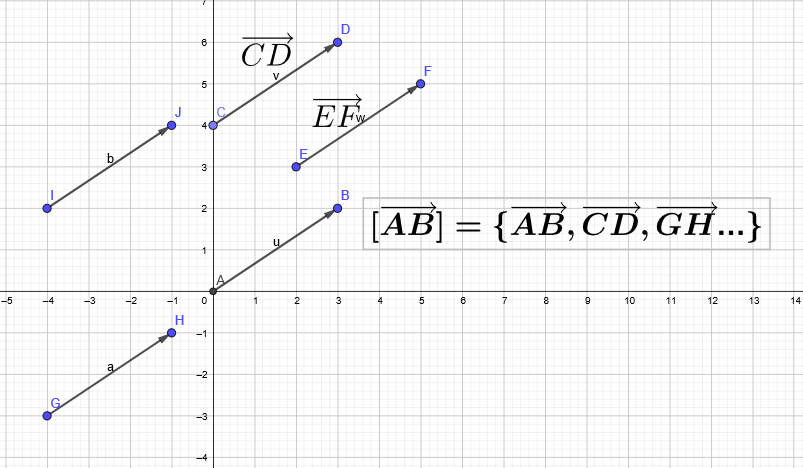
\includegraphics[width=0.9\textwidth]{img/Fijos-libres.png}
    \caption{Los diferentes vectores fijos de $V^2$ que tienen las mismas coordenadas forman parte del vector libre. 
    \newline
    De la misma manera que, la idea $\rfrac{1}{2}=\rfrac{2}{4}=\rfrac{3}{6}$ se escribiría, formalmente: $\left[\rfrac{1}{2}\right] = \left\{\rfrac{1}{2},\rfrac{2}{4},\rfrac{3}{6} ... \right\}$}
    \label{fig:plano}
\end{figure}


Denotaremos por $[\vec{AB}]$ al vector libre cuyas coordenadas son las del vector que va de $A$ a $B$.

Denotaremos por $\vec{AB}$ al vector fijo que va de $A$ a $B$.





\begin{defn}[Vector\IS definido por dos puntos]
(Página 278)

Dados dos puntos $A=(a_1,a_2,a_3)$ y $B = (b_1,b_2,b_3)$, tenemos 
    \begin{itemize}
        \item $\vec{AB} = \hide{(b_1-a_1, b_2-a_2, b_3-a_3)}$
        \item $\vec{BA} = \hide{(a_1-b_1, a_2-b_2, a_3-b_3)}$ 
    \end{itemize}
\end{defn}

\begin{proof}
Lo único que tenemos para trabajar son vectores de posición. 
%
En este caso son $\vec{a} = \vec{OA}$ y $\vec{b} = \vec{OB}$. 

Tenemos que $\vec{a} + \vec{AB} = \vec{b} \dimplies \vec{AB} = \vec{b}-\vec{a}$.
\end{proof}

\begin{example}
    Halla un vector definido por $A(1,0,3)$ y $B(2,1,2)$.
    
    \hide{\[\vec{AB} = (2-1, 1-0, 2-3) = (1,1,-1)\]}
\end{example}

\begin{problem}

Utilizando vectores de posición, demuestra que el punto medio entre los puntos $A$ y $B$, que llamamos $M_{AB}$, tiene por coordenadas:

\[M_{AB} = \left(\frac{a_1+b_1}{2},\frac{a_2+b_2}{2},\frac{a_3+b_3}{2}\right)\]

\ppart \textbf{Ampliación:} Dados los puntos $A(a_1,a_2,a_3)$ y $B(b_1,b_2,b_3)$, calcula las coordenadas del punto que divide el segmento $AB$ dejando $\rfrac{1}{3}$ de distancia con $A$ y $\rfrac{2}{3}$ de distancia con $B$. \textit{Pista: planteamiento parecido al punto medio.}

\solution

\[
\left\{
\begin{array}{c}
    \vec{AM} + \vec{MB} = \vec{AB}\\
    \vec{AM} = \vec{MB}\\
    \vec{OM} = ?
\end{array}\right\}
 \implies 
  2\vec{AM} = \vec{AB} \dimplies
  \]\[ 
  2\left(\vec{OM} - \vec{OA}\right) = \vec{AB} \dimplies
  2\vec{OM} = \vec{AB} + 2\vec{OA} = 
  \]\[
  2\vec{OM} = \left(
  b_1-a_1,
  b_2-a_2,
  b_3-a_3
  \right) + 
  \left(
  2a_1 - 0,
  2a_2 - 0,
  2a_3 - 0
  \right) = 
  \left(
  b_1+a_1,
  b_2+a_2,
  b_3+a_3
  \right)\]\[
  \vec{OM} = \left(
  \frac{b_1+a_1}{2},
  \frac{b_2+a_2}{2},
  \frac{b_3+a_3}{2}
  \right)
\]

\end{problem}

% \begin{problem}

% Dado el punto definido por el vector de posición $\vec{OP} = (1,1,1)$ en el sistema de referencia $\{(1,0,0), \mathcal{B} = \{u_1 = (1,0,1), u_2 = (0,2,1), u_3 = (0,0,4)\}\}$, expresa sus coordenadas en el sistema de referencia: 
% %
% $\{(1,1,0), \mathcal{B} = \{\vec{i},\vec{j},\vec{k}\}\}$

% \solution

% ¿Qué significa $\vec{OP} = (1,-2,3)$? Las coordenadas son los coeficientes de los vectores de la base, por lo tanto:

% \[
% P = (1,0,0) + 1·u_1 - 2·u_2+ 3·u_3  \dimplies (1,0,0) + 1·(1,0,1) - 2·(0,2,1)  + 3·(0,0,4) = (2,-4,11)
% \]

% Expresamos el vector $(2,-4,11)$ en el sistema de referencia pedido:

% $(2,-4,11) = (1,1,0) + \lambda_1\vec{i}+ \lambda_2\vec{j}+ \lambda_3\vec{k} \implies (\lambda_1,\lambda_2,\lambda_3) = (1,4,11)$

% \end{problem}

\begin{problem}

Dado el punto definido por el vector de posición $\vec{OP} = (1,1,1)$ en el sistema de referencia $S_1 = \{O_1(1,0,0), \mathcal{B} = \{u_1 = (1,0,1), u_2 = (0,2,1), u_3 = (0,0,4)\}\}$, expresa sus coordenadas en el sistema de referencia: 
%
$S_2=\{O_2(1,1,0), \mathcal{B} = \{\vec{i},\vec{j},\vec{k}\}\}$

\solution

En realidad $\vec{OP} = \vec{O_1P}$, por estar expresado en ese sistema de referencia. 

Entendemos que $O_1(1,0,0)$ no está expresado en función de la base de $S_1$.

¿Qué significa $\vec{O_1P} = (1,1,1)$? Las coordenadas son los coeficientes de los vectores de la base, por lo tanto, tomando $O(0,0,0)$ tenemos:

\[
\vec{OP} = \vec{OO_1} + \vec{O_1P} = (1,0,0) + 1·u_1 + 1·u_2+ 1·u_3  \dimplies\]
\[ (1,0,0) + 1·(1,0,1) +1 ·(0,2,1)  + 1·(0,0,4) = (2,2,6)
\]

Expresamos el vector $\vec{OP}=(2,2,6)$ en el sistema de referencia pedido:
\[\vec{OP} = (2,2,6) = (1,1,0) + \lambda_1\vec{i}+ \lambda_2\vec{j}+ \lambda_3\vec{k} \implies (\lambda_1,\lambda_2,\lambda_3) = (1,1,6) = \vec{O_2P}\]

\vspace{-0.3cm}
\paragraph{Plan b:} 
\[\vec{OP} = \vec{OO_2} + \vec{O_2P} \dimplies \vec{O_2P} = \vec{OP} - \vec{OO_2} = \underbrace{(2,2,6)}_{\ast} - \underbrace{(1,1,0)}_{\Delta} = (1,1,6)\]
\obs Para este planteamiento es \textbf{necesario} que los vectores que operamos (en este caso $\ast$ y $\Delta$) en coordenadas estén expresados en la \textbf{misma base}. 
%
En este caso, dicha base es la base canónica.

\vspace{-0.3cm}
\paragraph{Plan c: } No es necesario pasar por el origen $O(0,0,0)$, aunque pueda resultar más fácil de interpretar así. 

Podríamos haber empezado desde el principio haciendo un razonamiento parecido al plan b. Buscamos $\vec{O_2P}$ y sabemos $\vec{O_1P}$, por lo que podemos plantear:

\[
  \vec{O_1O_2} + \vec{O_2P} = \vec{O_1P} \dimplies \vec{O_2P} = \vec{O_1P} - \vec{O_1O_2}
\]

Como para poder hacer operaciones de vectores en coordenadas necesitamos la misma base, tenemos:

\[
  \vec{O_2P} = \vec{O_1P} - \vec{O_1O_2} = (\textcolor{red}{1},\textcolor{blue}{1},\textcolor{green}{1})_{S_1} - (0,1,0)_{SH} = (\textcolor{red}{1}\vec{u_1} + \textcolor{blue}{1}\vec{u_2} + \textcolor{green}{1}\vec{u_3}) - (0,1,0)
\]\[
  = 1·(1,0,1) +1 ·(0,2,1)  + 1·(0,0,4) - (0,1,0) = (1,1,6)
\]

\begin{itemize}
   \item $(0,1,0)_{SH}$ quiere decir "el vector $(0,1,0)$ expresado en el sistema de referencia habitual".
   \item $(1,1,1)_{S_1}$ quiere decir "el vector $(1,1,1)$ expresado en el sistema de referencia $S_1$".
 \end{itemize} 
\end{problem}


\subsection{La recta}

\obs Dado que la única manera que tenemos de determinar los puntos es a través de vectores de posición, utilizaremos $\vec{p} = (x,y,z)$ de forma equivalente a $[\vec{OP}]$ para referirnos a un punto cualquiera del plano, al que accedemos a través de su vector de posición.

Formas de determinar una recta:
\begin{enumerate}
  \item Un punto\footnote{O su vector de posición} y un vector director.
  \subitem 2 puntos (se reduce al caso anterior)
  \subitem Un punto y una condición de paralelismo (se reduce al primer caso)
  \item 2 planos secantes.
  \item Un punto y un plano perpendicular (se verá en geometría euclídea).
\end{enumerate}

Como todo con lo que vamos a trabajar son operaciones con vectores con coordenadas en un sistema de referencia, en realidad el punto de origen del sistema de referencia no es relevante. (Ver ejemplo \ref{example::origen_ref}).

\subsubsection{Ecuaciones de la recta}

La 
%
\concept[Ecuación de la recta\IS vectorial]{ecuación vectorial de la recta} $r$ determinada por el punto $A$, cuyo vector de posición es $\vec{a}$, con vector director $\vec{u_r} $  es $r : \vec{p} = \vec{a} + \lambda \vec{u_r}$, con $\lambda\in\real, \forall P\in\real$.
%
De esta manera quedan determinados los vectores de posición de todos los puntos de la recta $r$.

¿Es posible construir la recta sin ese parámetro $\lambda$? En realidad,
$$r : \vec{p} = \vec{a} + \lambda \vec{u_r}\dimplies \underbrace{r:\displaystyle \left\{
\begin{array}{c} 
  x = a_1 + \lambda u_1\\
  y = a_2 + \lambda u_2 \\ 
  z = a_3 + \lambda u_3
\end{array}\right\}}_{(1)} \implies \underbrace{r:\frac{x-a_1}{u_1} = \frac{y-a_2}{u_2} = \frac{z-a_3}{u_3}}_{(2)}$$

\begin{itemize}
    \item A $(1)$ lo denominamos \concept[Ecuación de la recta\IS paramétrica]{ecuación paramétrica de la recta}
    \item A $(2)$ lo denominamos \concept[Ecuación de la recta\IS continua]{ecuación continua de la recta}
\end{itemize}

\[
\frac{x-a_1}{u_1} = \frac{y-a_2}{u_2} = \frac{z-a_3}{u_3}\overset{(1)}{\implies} \left\{
\begin{array}{c}
     \displaystyle\frac{x-a_1}{u_1} = \frac{y-a_2}{u_2}\\
     \displaystyle\frac{y-a_2}{u_2} = \frac{z-a_3}{u_3}
\end{array}\right\} \implies
\underbrace{\left\{\begin{array}{cccc}
     Ax + &By    &     & = D\\
          &B'y   &+ C'z  & = D
\end{array}\right\}}_{(2)}
\]


\begin{figure}[hptb]
    \centering
    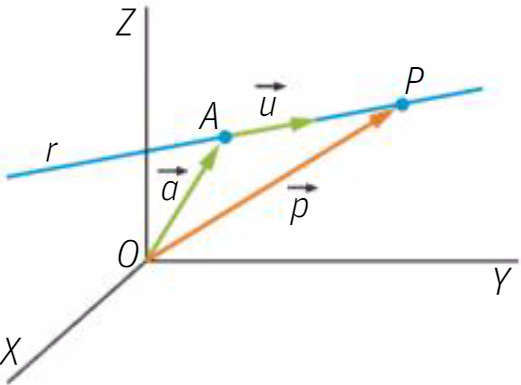
\includegraphics[width=0.4\textwidth]{img/EcVectorialRecta.png}
    \caption{Representación gráfica de la ecuación vectorial de la recta.}
    \label{fig:plano}
\end{figure}


Donde:
\begin{itemize}
    \item (1) \hide{Se han elegido estas 2 parejas, pero podrían haberse elegido otras, dando lugar a otras ecuaciones implícitas de la misma recta.}
    \item (2) \hide{\concept[Ecuación de la recta\IS implícita]{ecuación implícita de la recta}}
    \subitem \obs \hide{Si interpretáramos las ecuaciones implícitas de la recta como un sistema de ecuaciones, tendríamos un sistema compatible indeterminado con grado de libertad 1.}
    \subitem \obs La dimensión de la recta es 1.
\end{itemize}

\begin{problem}
    \ppart 
    Halla todas las ecuaciones de la recta que pasa por $A(0,1,2)$ y es paralela a la que pasa por $B(1,-2,-1)$ y $C(1,0,0)$
    \ppart 
    Halla un vector director de la recta $r:\displaystyle\frac{x-2}{1} = \frac{y-3}{5} = \frac{z-1}{4}$
    \ppart 
    Halla un vector director de la recta $r:\displaystyle\left\{\begin{array}{c} 2x+3y=4\\2x-y+3z=0\end{array}\right\}$
    \solution

\end{problem}

\textbf{Deberes:} 
\begin{itemize}
  \item Página 279.13,14.
  \item Página 281.18-21.
\end{itemize}

\subsection{El plano}

\subsubsection{Ecuaciones del plano}

Un plano queda determinado por \hide{un punto y dos vectores linealmente independientes}

La 
%
\concept[Ecuación del plano\IS vectorial]{ecuación vectorial del plano} 
%
$\pi$ determinada por el punto $A$ y los vectores linealmente independientes $\vec{V_{\pi}}$ y $\vec{W_{\pi}}$  es $r : \vec{p} = \vec{A} + \lambda \vec{V_{\pi}} + \mu\vec{W_{\pi}}$, con $\lambda\in\real$. De esta manera quedan determinados los vectores de posición de todos los puntos del plano.

Como en el caso de la recta, podemos escribir esta ecuación en forma de sistema con parámetros:

$$\pi : \vec{p} = \vec{A} + \lambda \vec{V_{\pi}} + \mu\vec{W_{\pi}}\dimplies \underbrace{\pi:\displaystyle \left\{\begin{array}{c} x = a_1 + \lambda v_1 + \mu w_1\\y = a_2 + \lambda v_2 + \mu w_2 \\ z = a_3 + \lambda v_3 + \mu w_3 \end{array}\right\}}_{(1)} $$

 A $(1)$ lo denominamos \concept[Ecuación del plano\IS paramétrica]{ecuación paramétrica del plano}

\[
\pi:\displaystyle \left\{
\begin{array}{c} 
x - a_1 = \lambda v_1 + \mu w_1\\
y - a_2 = \lambda v_2 + \mu w_2 \\ 
z - a_3 = \lambda v_3 + \mu w_3 
\end{array}\right\}
\]
Como los vectores $\vec{v},\vec{w}$ son linealmente independientes y el vector $AX$ es una combinación lineal de los otros 2 (ver \ref{fig:plano}, tenemos:

\[
\left|
\begin{array}{ccc} 
x - a_1 & v_1 & w_1\\
y - a_2 & v_2 & w_2 \\ 
z - a_3 & v_3 & w_3 
\end{array}\right| = 0
\]

Desarrollando esta ecuación, tendríamos una ecuación del tipo $Ax+By+Cz + D = 0$, que llamamos \concept[Ecuación del plano\IS implícita]{Ecuación implícita del plano}.


\begin{figure}[hptb]
    \centering
    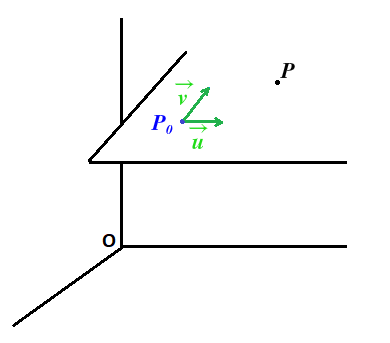
\includegraphics[width=0.65\textwidth]{img/ecplanos.png}
    \caption{Plano generado por un punto y dos vectores}
    \label{fig:plano}
\end{figure}

\begin{problem}
    \textbf{Calcula las ecuaciones del plano que pasa por los puntos $A(1,1,1), B(2,2,2), C(1,2,3)$}

    \solution 

    \hide{
    El primer paso sería calcular 2 vectores linealmente independientes de estos 3 puntos, para comprobar que los 3 puntos forman un plano (y no una recta).

    $\vec{AB} = (1,1,1) \quad\quad \vec{AC} = (0,1,2)$, que son linealmente independientes al no ser proporcionales.

    Ecuación vectorial: $\pi: \vec{p} = (1,1,1) + \mu\vec{AB} + \lambda\vec{AC}, \lambda,\mu\in\real$

    Ecuación paramétrica: $
    \displaystyle\left\{ \begin{array}{c}
      x = 1 + \mu\\
      y = 1 + \mu + \lambda\\
      z = 1 + \mu + 2\lambda
    \end{array} \right\}\text{ con } \lambda,\mu\in\real$

    Ecuación implícita: 

    \[
      \displaystyle \begin{vmatrix}
      x - 1 & 1 & 0\\
      y - 1 & 1 & 1\\
      z - 1 & 1 & 2\\
    \end{vmatrix} = 0 \dimplies \cdots \dimplies x - 2y+z=0
    \]
    }
\end{problem}


\begin{problem}
\ppart Halla la ecuación de 2 rectas que pertenezcan al mismo plano.
\ppart Halla un vector director del plano: $\pi_1: x+y+z = 3$
\ppart Halla el plano paralelo a $\pi_2: x+y+z = 3$ que pase por el origen de coordenadas.
\ppart Halla el plano paralelo al $XY$ que pasa por $A(-1,2,-2)$.
\obs Llamamos plano $XY$ al plano "del suelo", es decir, al plano $z=0$.

\ppart Página 283, ejercicios 25-28.

\solution

\end{problem}

\subsection{Posiciones relativas}

\subsubsection{Entre 2 planos}  

\begin{framed}
\textbf{Ecuaciones vectoriales o paramétricas:}
  \begin{itemize}
    \item Si 2 planos comparten 3 puntos, entonces son el mismo plano.
    \item Si los 4 vectores directores de los 2 planos son linealmente independientes, entonces los planos son secantes en un punto.
    \item Si la matriz formada por los 4 vectores directores de los 2 planos tiene rango 3, los planos son secantes en una recta.
    \item Si la matriz formada por los 4 vectores directores de los 2 planos tiene rango 2, los planos son paralelos.
    \item Si 2 planos paralelos comparten un punto, entonces son coincidentes.
  \end{itemize}
\end{framed}



\subparagraph{Ecuaciones implícitas}

\[
\left\{\begin{array}{c}
\pi_1: Ax+By+Cz = D\\
\pi_2: A'x+B'y+C'z = D'
\end{array}\right\}
\]

Obtenemos las matrices: $M = \displaystyle\begin{pmatrix}A&B&C\\A'&B'&C'\end{pmatrix}$ y $M^* = \displaystyle\begin{pmatrix}A&B&C&D\\A'&B'&C'&D'\end{pmatrix}$

\begin{framed}
  \begin{itemize}
    \item $Rg(M) = Rg(M^*) = 1 $\hide{ coincidentes.}
    \item $Rg(M) < Rg(M^*) = 2 $\hide{ paralelos.}
    \item $Rg(M) = Rg(M^*) = 2 $\hide{ secantes.}
  \end{itemize}
\obs En realidad, sería como las ecuaciones implícitas de la recta.
\end{framed}

\subsubsection{Entre 3 planos}

\subparagraph{Ecuaciones vectorial o paramétricas}

Se pasa a implícitas.

\subparagraph{Ecuaciones implícitas}
\[
\left\{\begin{array}{c}
\pi_1: Ax+By+Cz = D\\
\pi_2: A'x+B'y+C'z = D'\\
\pi_3: A''x+B''y+C''z = D''\\
\end{array}\right\}
\]

Obtenemos las matrices: 
$M  = \displaystyle\begin{pmatrix}
A&B&C\\
A'&B'&C'\\
A''&B''&C''
\end{pmatrix}
$ y 
$M^* = \displaystyle\begin{pmatrix}
A&B&C&D\\
A'&B'&C'&D'\\
A''&B''&C''&D''
\end{pmatrix}
$

Las posibilidades son: (ver figura \ref{fig:PosicionesRelativasPlanos})
\begin{framed}
  \begin{itemize}
    \item $Rg(M) = Rg(M^*) = 1 $\hide{ SCI, secantes en un plano [grado de indeterminación 2, por lo que hay dos parámetros. \textbf{Coincidentes}.}
    \item $Rg(M) < Rg(M^*) = 2 $\hide{ paralelos.}
    \item $Rg(M) = Rg(M^*) = 2 $\hide{ SCI, secantes en una recta [grado de indeterminación 1, por lo que hay un parámetro.}
    \item $Rg(M) = 2 < Rg(M^*) = 3 $\hide{ no se cortan los 3. Sistema incompatible}
    \item $Rg(M) = Rg(M^*) = 3 $\hide{ SCD, secantes en un punto que es la solución del sistema.}
  \end{itemize}  
\end{framed}

\begin{figure}[hptb]
    \centering
    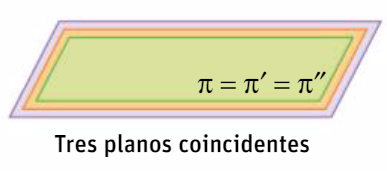
\includegraphics[width=0.65\textwidth]{img/Captura1.png}
    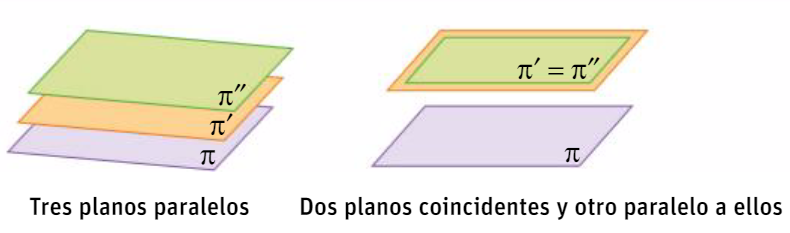
\includegraphics[width=0.95\textwidth]{img/Captura2.png}
    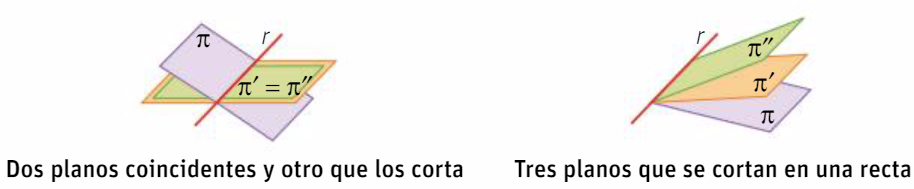
\includegraphics[width=1.1\textwidth]{img/Captura3.png}
    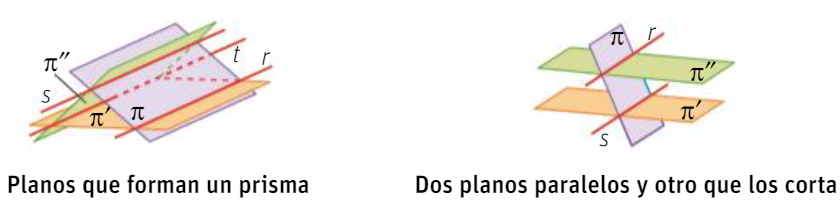
\includegraphics[width=1.1\textwidth]{img/Captura4.png}
    \caption{Representación gráfica de las posiciones relativas de 3 planos.}
    \label{fig:PosicionesRelativasPlanos}
\end{figure}




\subsection{Posiciones relativas entre recta y plano}

\paragraph{Ecuaciones implícitas: } si tanto la recta como el plano están dados en ecuaciones implícitas, estaríamos en la posición relativa de 3 planos, sabiendo que 2 de ellos son secantes en una recta.

\paragraph{Ecuaciones paramétrica: } $\pi: \{P_{\pi},\vec{v_{\pi}}, \vec{w_{\pi}}\}$ 

\begin{center}
\begin{tabular}{ccc}
$P_r \in \pi $ & $\vec{v_r}$ LD de $v_{\pi}, \vec{w}_{\pi}$ & Conclusión\\
No & No & Secantes en un punto\\
No & Sí & Recta paralela\\
Sí & No & Secantes en un punto\\
Sí & Sí & Recta contenida en el plano\\
\end{tabular}
\end{center}

\paragraph{Plano implícito, recta paramétrica: } comprobamos si existe algún valor de $\lambda_{r}$ para el que se cumpla la ecuación implícita del plano. 
\begin{itemize}
  \item $\exists!\lambda \implies $ secante.
  \item $\lambda \in \real \implies$ contenida.
  \item $\not\exists \lambda \implies $ paralela.
\end{itemize}

Deberes: Hoja resumen de teoría,105ab,107ab

\subsubsection{Posiciones relativas entre 2 rectas:}

Dadas las rectas 
$r:\vec{p} = \vec{a} + \lambda\vec{u},\quad \lambda\in\real$
y
$s:\vec{p} = \vec{b} + \lambda\vec{w},\quad \lambda\in\real$. 

Si los vectores directores son paralelos (proporcionales), las rectas pueden ser paralelas o coincidentes. 
%
Para poder distinguir , podríamos ver si un vector formado por un punto de cada recta es también proporcional (entonces serían coincidentes) o si no (entonces serían secantes).

De la misma manera, si los vectores son linealmente independientes las rectas pueden cruzarse o cortarse. 
%
Para distinguir estos 2 casos, podríamos ver si un vector formado por un punto de cada recta es linealmente dependiente a los otros 2 (entonces serían secantes porque formarían un plano que contiene al vector) o si no (entonces se cortarían en el espacio).

Así, buscamos estudiar la dependencia lineal de los 2 vectores directores ($\vec{u},\vec{w}$) y de los 2 vectores directores respecto de un vector formado, arbitrariamente, con 2 puntos de las rectas ($\vec{AB}$, con $A(a_1,a_2,a_3)\in r$ y $B(b_1,b_2,b_3)\in s$). 
%
Para ello, formamos las matrices:

$M  = \displaystyle\begin{pmatrix}
u_1&w_1\\
u_2&w_2\\
u_3&w_3
\end{pmatrix}
$ y 
$M^* = \displaystyle\begin{pmatrix}
u_1&w_1&b_1-a_1\\
u_2&w_2&b_2-a_2\\
u_3&w_3&b_3-a_3\\
\end{pmatrix}
$

\begin{framed}
  \begin{itemize}
    \item $Rg(M) = Rg(M^*) = 1 $\hide{ SCI, secantes en una recta [grado de indeterminación 1, por lo que hay dos parámetros. \textbf{Coincidentes}.]}
    \item $Rg(M) = 1 < Rg(M^*) = 2 $\hide{ paralelas.} 
    \item $Rg(M) = Rg(M^*) = 2 $\hide{ SCI, secantes en un plano [dimensión 2]. $\vec{AB}$ se puede escribir como combinación lineal de $\vec{u}$ y $\vec{w}$}
    \item $Rg(M) = 2 < Rg(M^*) = 3 $\hide{ se cruzan en el espacio.} 
  \end{itemize}  
\end{framed}
\obs También se podría trabajar con las matrices traspuestas si uno está más familiarizado con estudiar el rango como combinaciones lineales de filas en lugar de columnas.

\begin{problem}
Página 289, ejercicios 52, calculando puntos de cortes
\solution

\end{problem}


\subsubsection{Haz (no se pide en selectividad, así que se salta)}
\paragraph{Haz de rectas paralelas: } cambia el punto, manteniendo fijo el vector. 
\paragraph{Haz de rectas secantes: } cambia el vector (sin ser nunca nulo), mantiene fijo el punto.
\paragraph{Haz de planos paralelelos: } cambia el punto, mantiene los vectores
\paragraph{Haz de planos secantes en una recta: } mantiene un vector y un punto, cambia el otro vector.

\begin{problem}
Tema 11: 56,57,59,60.
\solution
\end{problem}

Deberes: 118,136,143

\subsubsection{Practicamos en general}

Tema 11: 
122,127,130,134,135,136,139,140,143,145,149,150

Tema 11:
\begin{itemize}
  \item Básicos: 83,91,92,93a,98,100,101a,103a,104a,105,106,107d,108
  \item Síntesis: 111-119
  \item Completos: 122-124,127,129-133
\end{itemize}




\section{Geometría euclídea (del 25/01 al final)}

Llamamos geometría euclídea al espacio en el que podemos medir, cosa que hasta ahora no era posible.

Todo surge desde el módulo de un vector. Llamamos \concept[Módulo de un vector]{módulo de un vector} a la longitud que tiene. Dado $\vec{v}$, se define el módulo como $|\vec{v}|$.

\subsection{Producto, escalar, vectorial y mixto}

\paragraph{Introducción sobre el origen del producto escalar y vectorial}

Fuentes consultadas:
\begin{itemize}
  \item \href{http://www.suitcaseofdreams.net/Geometric_multiplication.htm}{Relación forma polar y binómica del producto complejo}
  \vspace{-0.4cm}
  \item \href{https://www2.clarku.edu/faculty/djoyce/complex/mult.html}{Interpretación geométrica del producto complejo}
  \vspace{-0.4cm}
  \item \href{https://www.quora.com/Who-invented-the-dot-product-and-cross-product}{Historia y aplicación de los cuaterniones los productos}
  \vspace{-0.4cm}
  \item \href{https://es.wikipedia.org/wiki/Cuaterni%C3%B3n}{ Extensión de los complejos al grupo de los quaterniones}
\end{itemize}

Dados 2 números complejos $z_1 = a_1+b_1i$, $z_2 = a_2+b_2i$. Expresando estos números complejos en forma polar tenemos: $z_1=r_{\alpha_1}$ y $z_2 = s_{\alpha_2}$.  

$z_1·z_2 = (a_1a_2 - b_1b_2) + (a_1b_2+a_2b_1)i = r·s_{\alpha_1+\alpha_2}$.

Tomando $z_1·\bar{z_2} = (a_1a_2 + b_1b_2) + (a_1b_2-a_2b_1)i = r·s_{\alpha_1-\alpha_2}
$

\subparagraph{Estudio de la parte real (producto escalar)}

En $Re(z_1·\bar{z_2}) = a_1a_2 + b_1b_2 = Re(r·s_{\alpha_1-\alpha_2})$

Para calcular $Re(r·s_{\alpha_1-\alpha_2}) = Re(r·s·\cos(\alpha_1-\alpha_2) + i·r·s·\sen(\alpha_1-\alpha_2)$, por lo que podemos completar:

$ a_1a_2 + b_1b_2 = |z_1||z_2|·\cos(\alpha_1-\alpha_2)$, y, siendo conscientes que $\alpha_1-\alpha_2$ es el ángulo que forman los 2 vectores, obtenemos la expresión del producto escalar de 2 vectores.


\subparagraph{Estudio de la parte imaginaria (producto vectorial)}

Al extender este razonamiento al grupo de los cuaterniones, tendríamos:

\newcommand{\quat}{\vec}

$Re(z_1\bar{z_2}) = Re\left((b_1\quat{i}+c_1\quat{j}+d_1\quat{k})·(-b_2\quat{i}-c_2\quat{j}-d_2\quat{k})\right) = (b_1b_2+c_1c_2+d_1d_2)$

Lo espectacular viene al considerar la parte "imaginaria" (aunque no tengamos claro cómo se define ese concepto en los cuaterniones):

$Im(z_1\bar{z_2}) = f(\quat{i},\quat{j},\quat{k})$, cuya expresión analítica es la del producto vectorial, ya que en grupo de los cuaterniones $\quat{i}\quat{j}=\quat{k}$ y todo eso.

\subsubsection{Producto escalar}

\begin{itemize}
  \item Definición.
  \item Base ortogonal y ortonormal.
  \item Expresión analítica.
  \item Cálculo del módulo (porque Pitágoras tridimensional no funciona).
  \item Base canónica.
  \item Interpretación geométrica (proyección).
\end{itemize}

\subsubsection{Producto vectorial}
\begin{itemize}
  \item Definición.
  \subitem Regla de la mano derecha
  \item Expresión analítica.
  \item Interpretación geométrica. 
\end{itemize}


\subsubsection{Producto mixto}

\begin{itemize}
  \item ¿Qué ocurre si en el producto vectorial meto un vector en lugar de $\vec{i},\vec{j},\vec{k}$?
  \item Definición.
  \item Expresión analítica.
  \item Interpretación geométrica. 
\end{itemize}

\subsubsection{Practicamos en general ejercicios del tema 9}

\subsection{Aplicación de los productos}

\subsubsection{Vector normal del plano}
\subsection{Perpendicular común}

\subsection{Proyecciones y medidas}
\subsubsection{Simetría de un punto respecto de otro punto}
\subsubsection{Simetría de un punto respecto de una recta}
\subsubsection{Simetría de un punto respecto de un plano}

\newpage
\subsection{Ángulos}
\subsubsection{Ángulo formado por dos rectas: secantes, se cruzan y paralelas/coincidentes}
\subsubsection{Ángulo formado por dos planos}
\subsubsection{Ángulo formado por recta y plano}

\subsection{Distancias}
\subsubsection{Entre 2 puntos}
\subsubsection{Plano mediador}
\subsubsection{Entre punto y plano}
\subsubsection{Planos bisectores}
\subsubsection{Entre 2 planos}
\subsubsection{Entre recta y plano}
\subsubsection{Entre punto y recta}
\subsubsection{Entre 2 rectas paralelas}
\subsubsection{Entre 2 rectas no paralelas}

\subsubsection{Volumen del paralelepípedo}
